\documentclass{article}
\usepackage{graphicx}
\usepackage[utf8]{inputenc}


\title{EECS 31L Midterm Project: \\ Enhanced Arithmetic Logic Unit Implementation in SystemVerilog}
\author{Group: Um \\ Kathy Nguyen (49131012), Josh Park (25729974), Aina Tancinco (66726318),\\ Nicole Thai (55729939), Amy Yee (55246967) }
\date{30 October 2017}

\begin{document}

\maketitle

\section{Introduction}

Our Enhanced Arithmetic Logic Unit (ALU) consists of 12 operations that are selected through a multiplexer: addition, subtraction, increment, decrement, move, 1-bit logical shift left of A, SIMD Add (four 8-bits add), bitwise AND, bitwise OR, bitwise XOR, complement, and 2's complement. The multiplexer implements a conditional statement to properly determine which module to call on depending on the opcode selected. All 12 operations selected are passed to determine the proper call to its corresponding module implementation of the operation. This design and simulation of an Enhanced ALU will be connected to the FPGA board for analysis of the functions on the board.

\subsection{32-Bit Enhanced ALU Block Diagram}
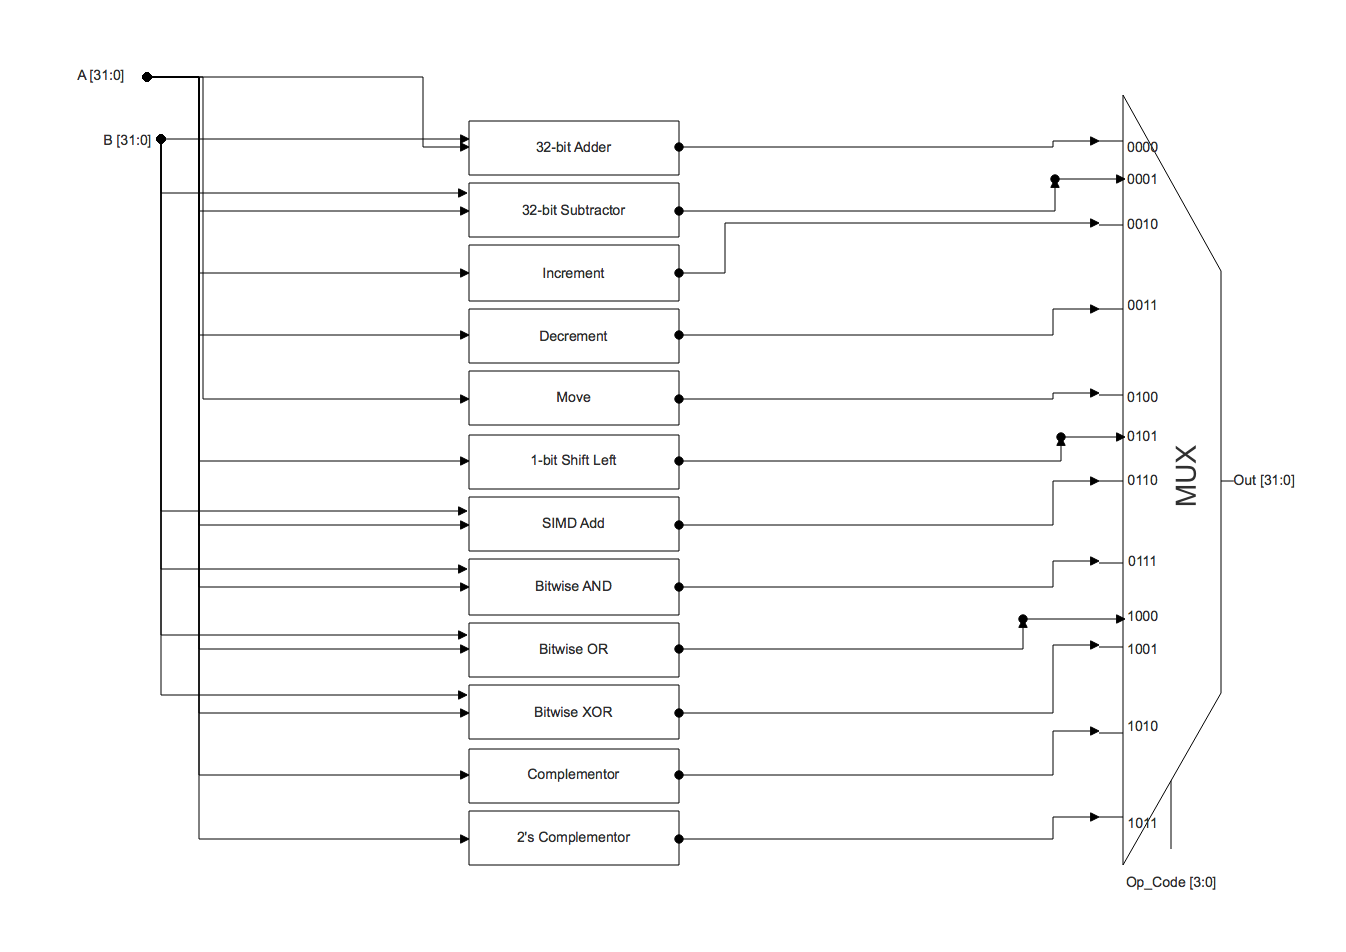
\includegraphics[scale=.5]{photos/ALUBlockDiagram} 
\break

\section{Process}
Through effective collaboration, the Um group divided the task of implementation of an ALU into twelve modules among five members of the group. Individually the UM group struggled; however the UM group would collaborate on specific submodules that were a bit more challenging such as the addition and subtraction module when handling errors mentioned in more details below. Collectively, we were able to collaborate to increase efficiency and catch potential errors in the code. The multiplexer connects 12 submodules by selecting them based on the conditional statement that would call the specific submodule.

\subsection{Addition}
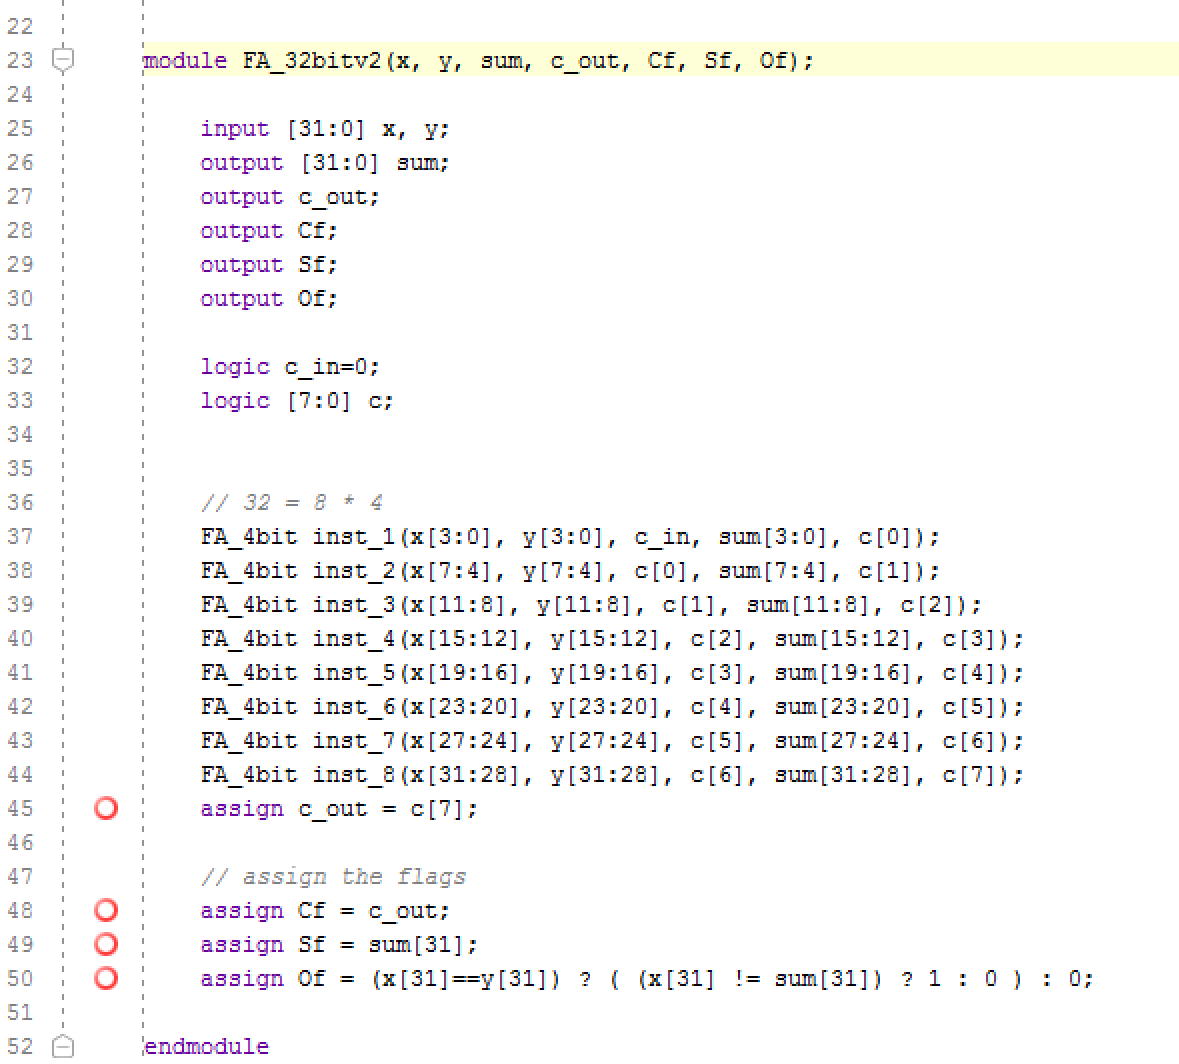
\includegraphics[scale=0.5]{photos/32bit_adder_code}
\break
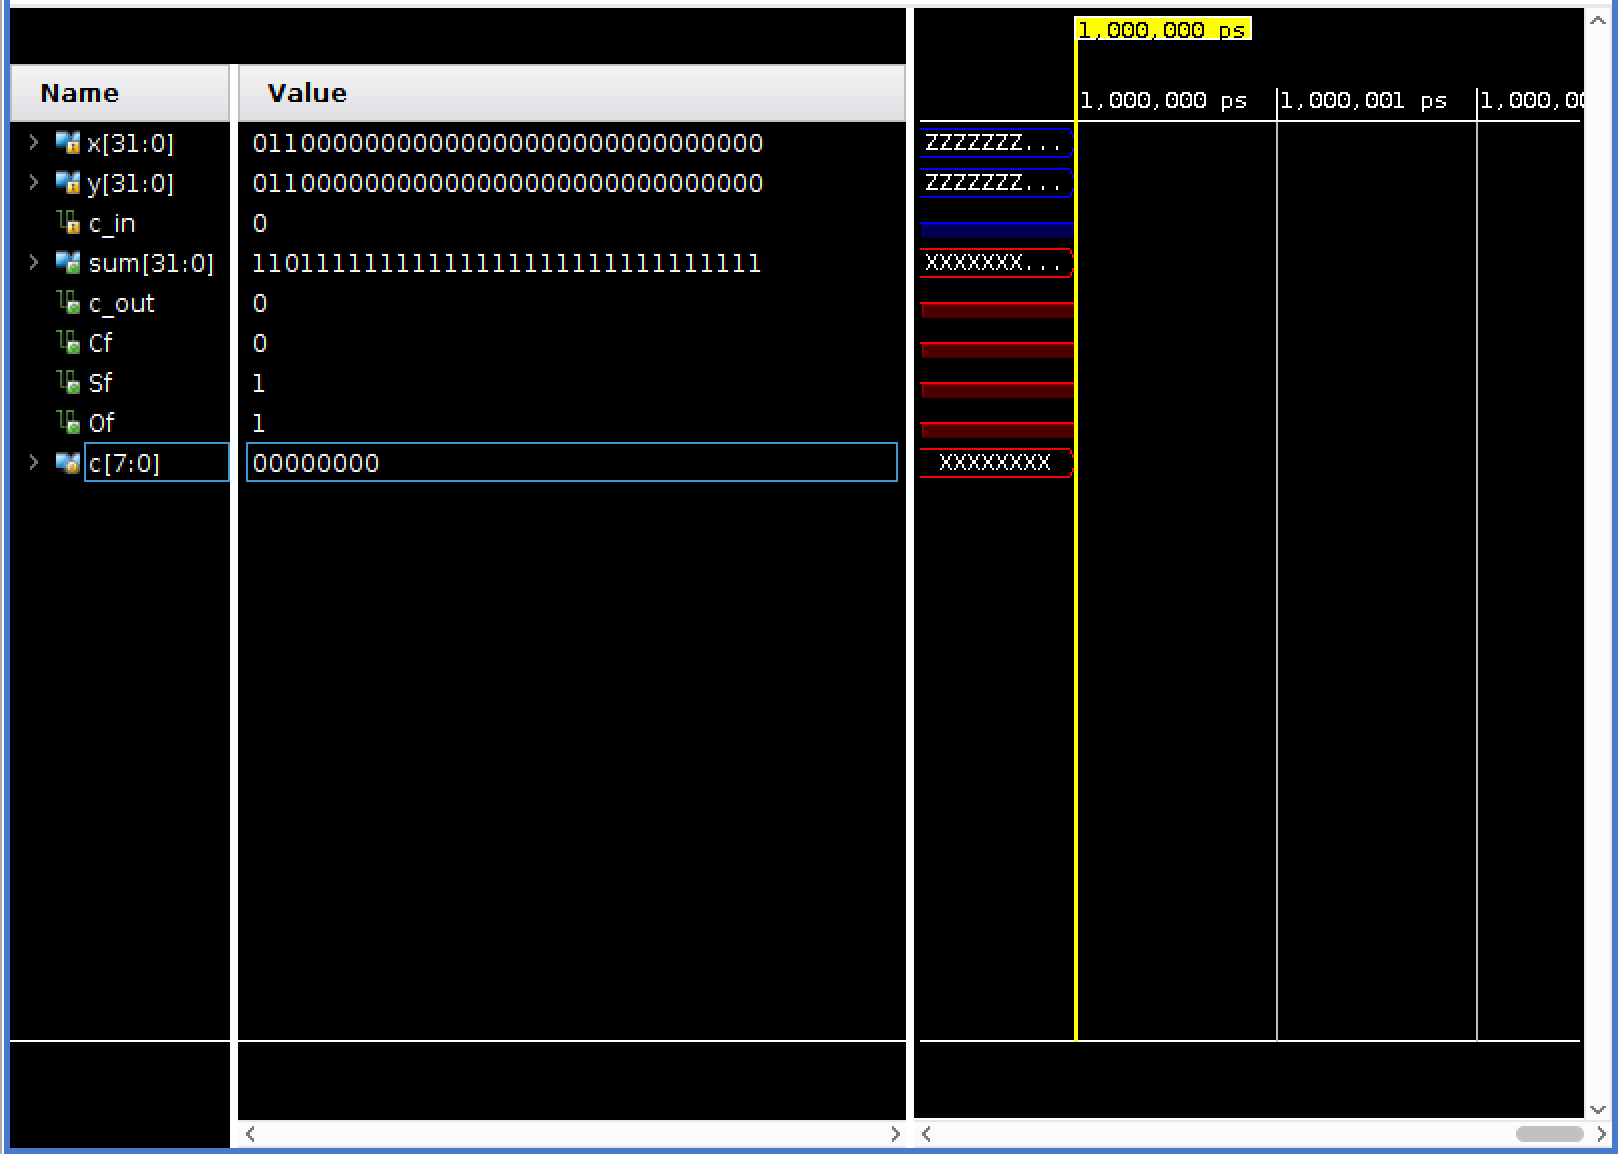
\includegraphics[scale=0.24]{photos/32bit_adder_boundary1}
\break
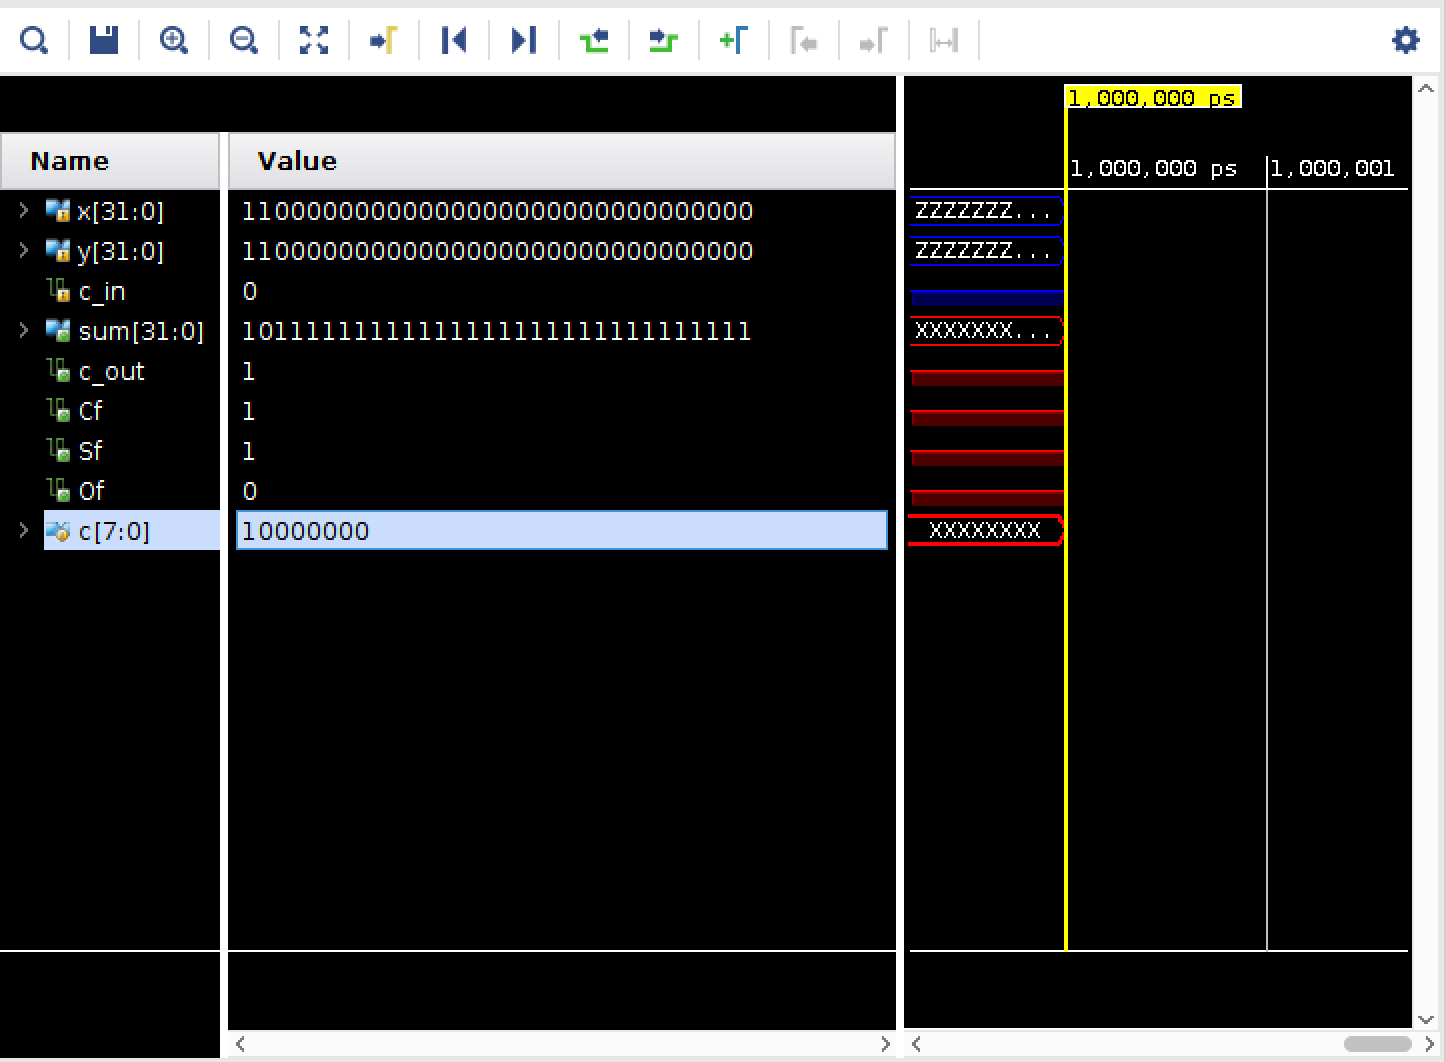
\includegraphics[scale=0.24]{photos/32bit_adder_boundary2}
\break

The Um group initially began typing out the bit-by-bit equation that we were provided in lab for our 4 bit full adder. However, the module was seemingly inefficient therefore module instantiation was utilized instead. The 32 bit adder module utilizes the 4 bit adder module from lab 2 and instatiates the 4 bit adder 8 times. Although the mistype of an equation in the 4 bit adder module prevented us from executing the 32 bit adder successfully, the answer was made clear eventually. This error made module instantiation the obvious approach as it made miniscule typing errors less likely. In addition, the importance of keeping track of the carry outs and being able to track it from the least significant bit all the way to the most significant bit were made obvious when we realized we needed to determine the different flags. The overflow flag was determined using conditional statements according to the logical interpretation for overflow cases. To test the flags, forced constants such as \{0110,28'b0\} and \{1100,28'b0\} were added to ensure that the carry and overflow flags were triggered for appropriate cases. We continued to test values in the lower range including unsigned decimals less than 100. After multiple successful executions, the 32 bit adder was determined to be complete.

\subsection{Subtraction}
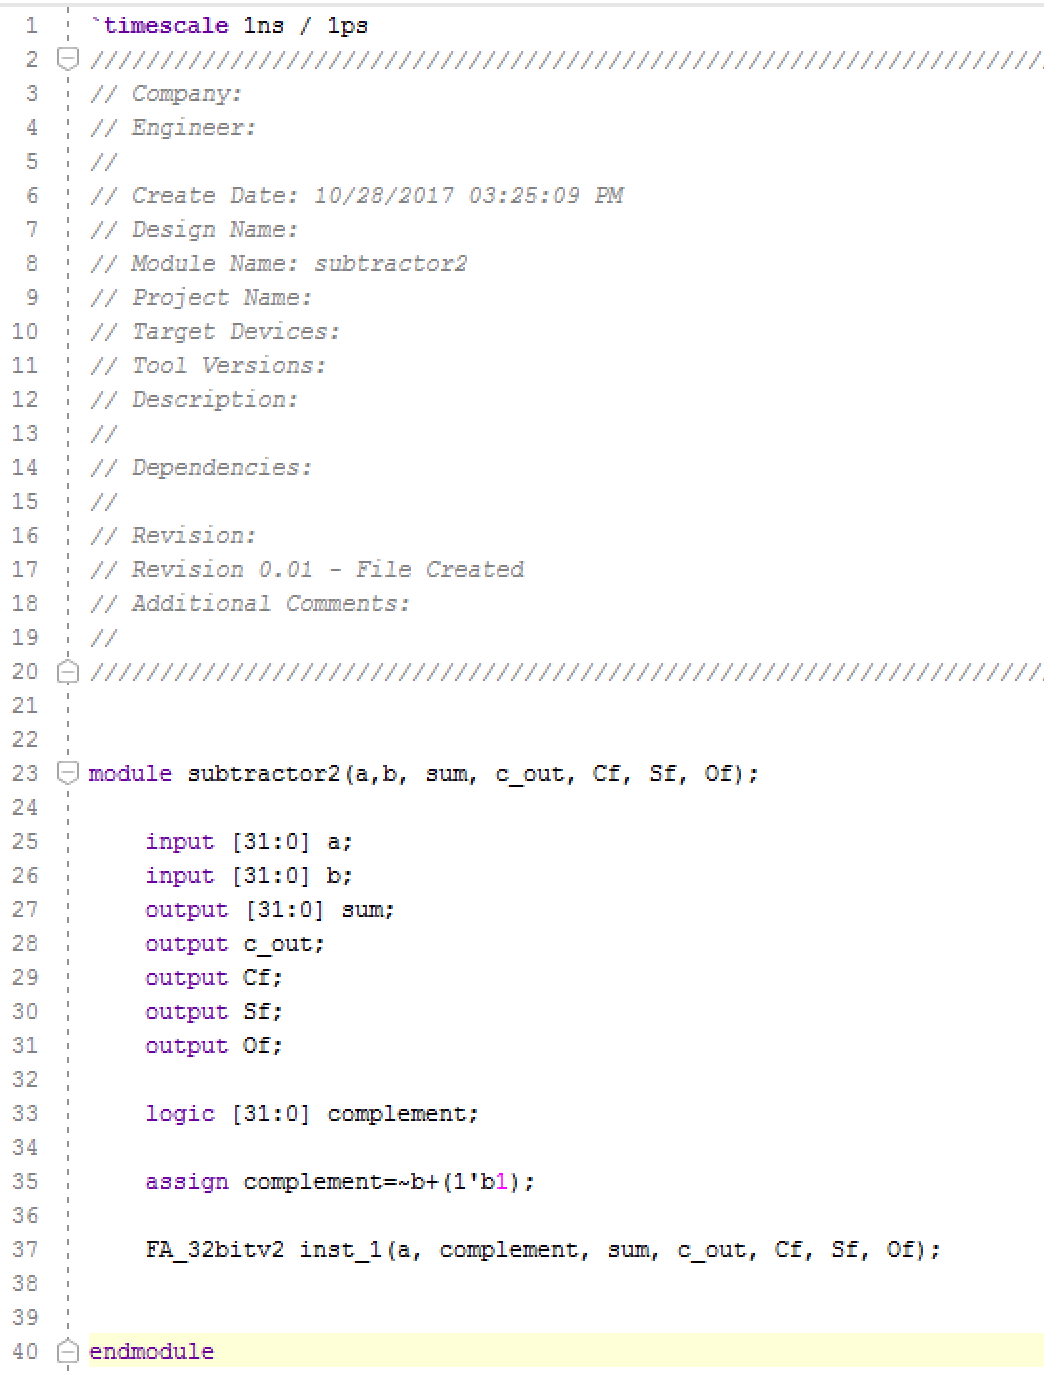
\includegraphics[scale=0.5]{photos/subtractor_code}
\break
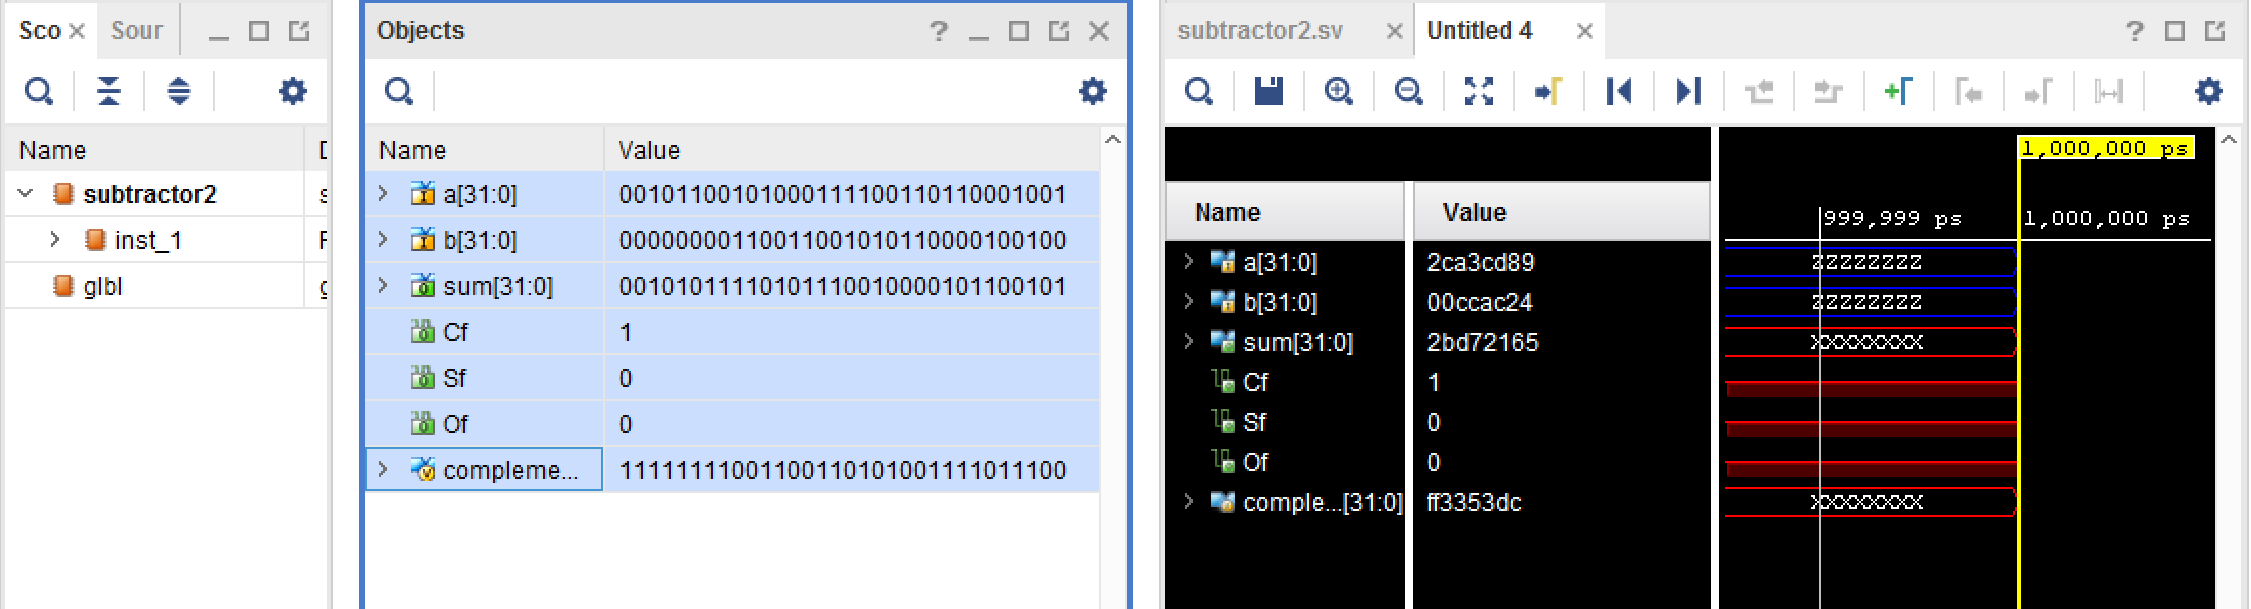
\includegraphics[scale=0.41]{photos/subtractor_simulation}
\break
Because subtraction is just the addition of the first given number and the two's complement of the other, using module instantiation of the previous 32 bit adder seemed more efficient. Two's complement was performed on the second input value for the subtraction operation. This value was stored into a separate variable called complement since this made it easier to see if the initial value properly underwent the two's complement operation. After this, the two values, A and complement were added using an instantiation of the 32-bit adder. The final result would be the different between A and B, and is stored into the "Out" return variable in the main module. Carry and Sign Flags were determined the same way it was in the 32-bit Adder, and was tested with the following cases:
00000101110000001111100001011000 and 00010001000100010001000100010001, 32'hffffffff and 32'hffffffff, 32'h0000eeee and 32'heeee0000.

\subsection{Increment}
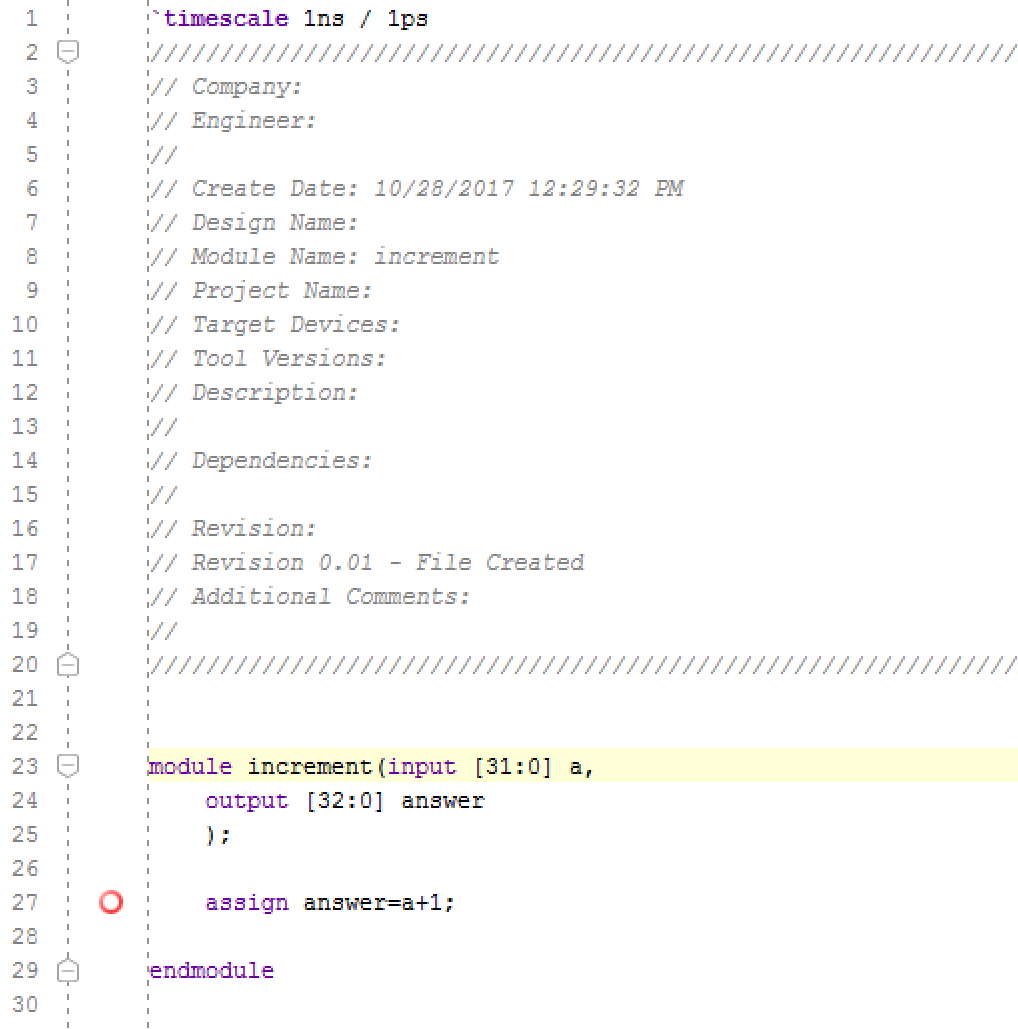
\includegraphics[scale=0.5]{photos/increment}
\break
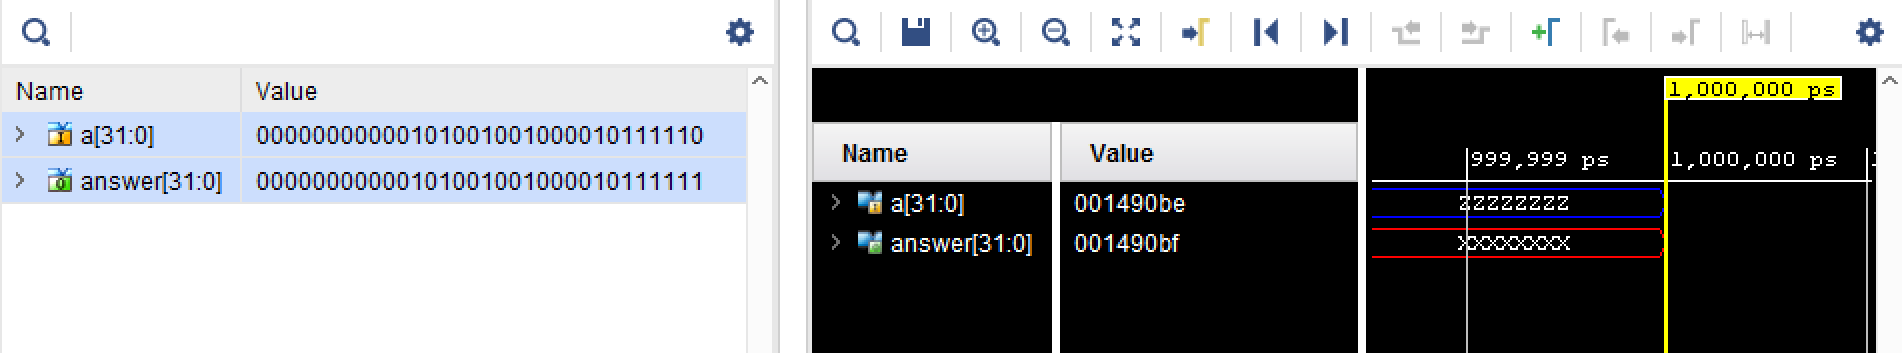
\includegraphics[scale=0.49]{photos/increment_simulation}
\break
Increment adds 1 to the 32-bit user input and returns the value after incrementing by 1.In SystemVerilog, the input [31:0] A the user entered is 00000037, so the expected output [32:0] answer would be 00000038. The reason the array goes from [31:0] to [32:0] is to handle overflow that would occur when adding 1. We made it more efficient by making it one line. 

\subsection{Decrement}
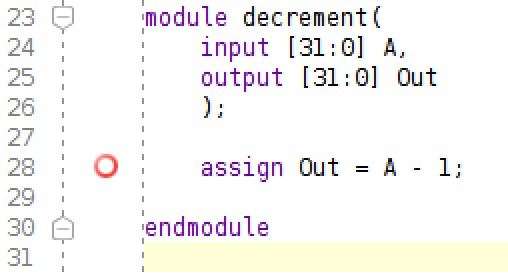
\includegraphics[scale=.5]{photos/decrement}
\break
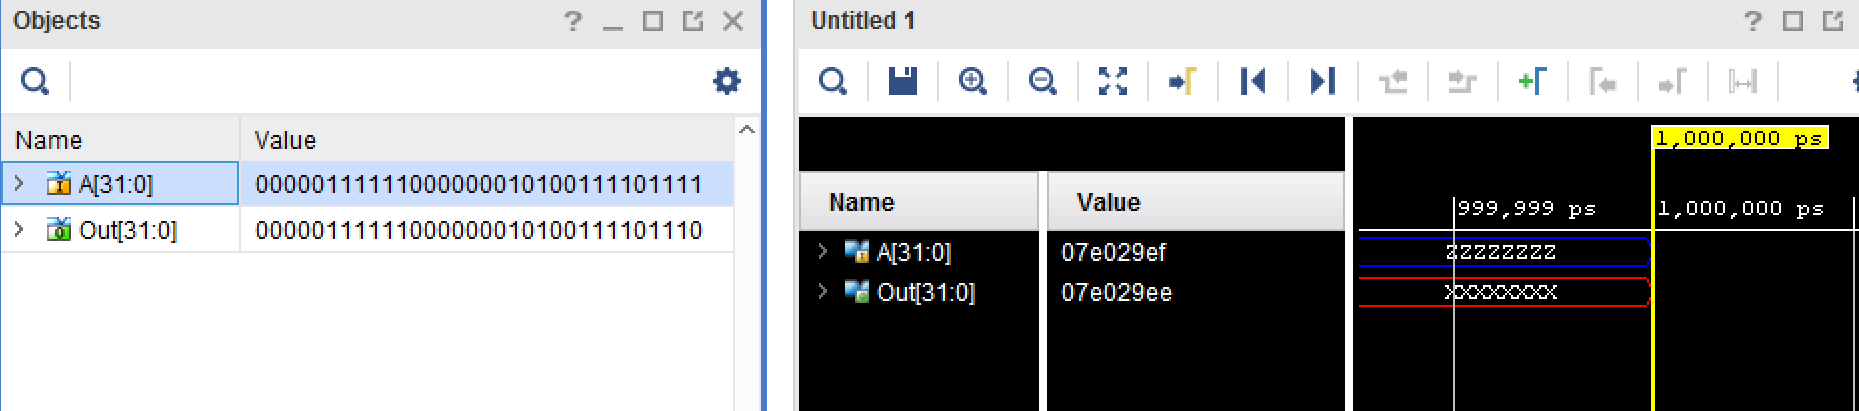
\includegraphics[scale=.5]{photos/decrement_simulation}
\break
Decrement subtracts user input by 1 and returns the decrement. In SystemVerilog, the hexadecimal input [31:0] A the user entered was 0000000f, so the expected output [31:0] Out would be 0000000e when subtracting by 1. 

\subsection{Move}
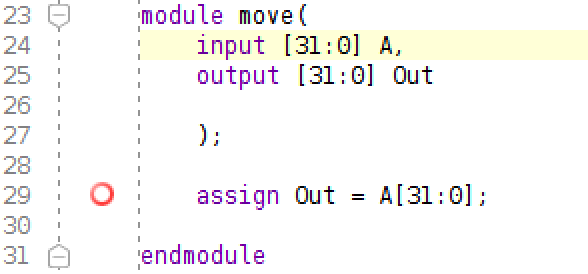
\includegraphics[scale= .5]{photos/move}
\break
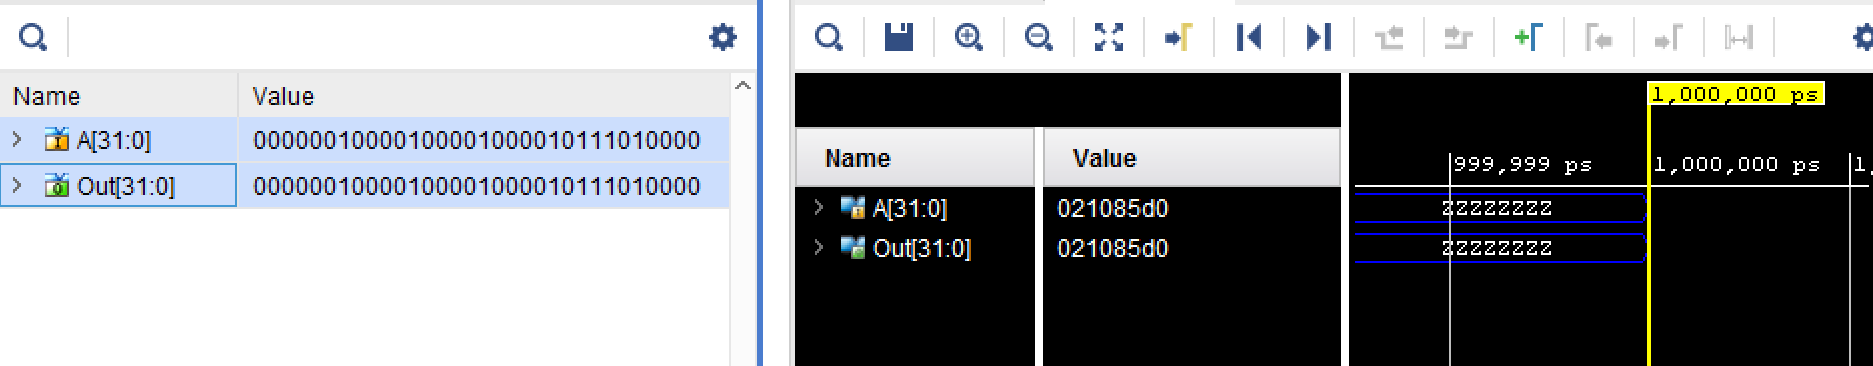
\includegraphics[scale= .5]{photos/move_simulation}
\break
The Move function takes an input and moves it to the output. This is implemented in SystemVerilog by defining an input port and output port. The input receives a 32-bit binary number then assigns it to the output port.

\subsection{1-bit Logical Shift Left of A}
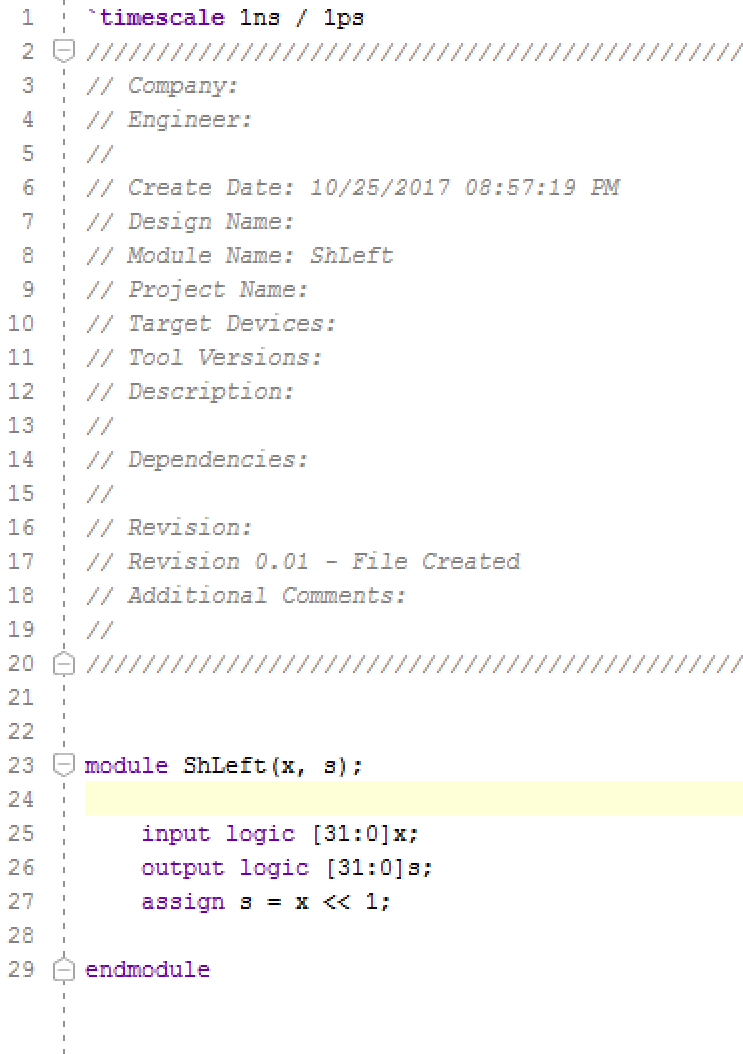
\includegraphics[scale=0.5]{photos/shleft_code}
\break
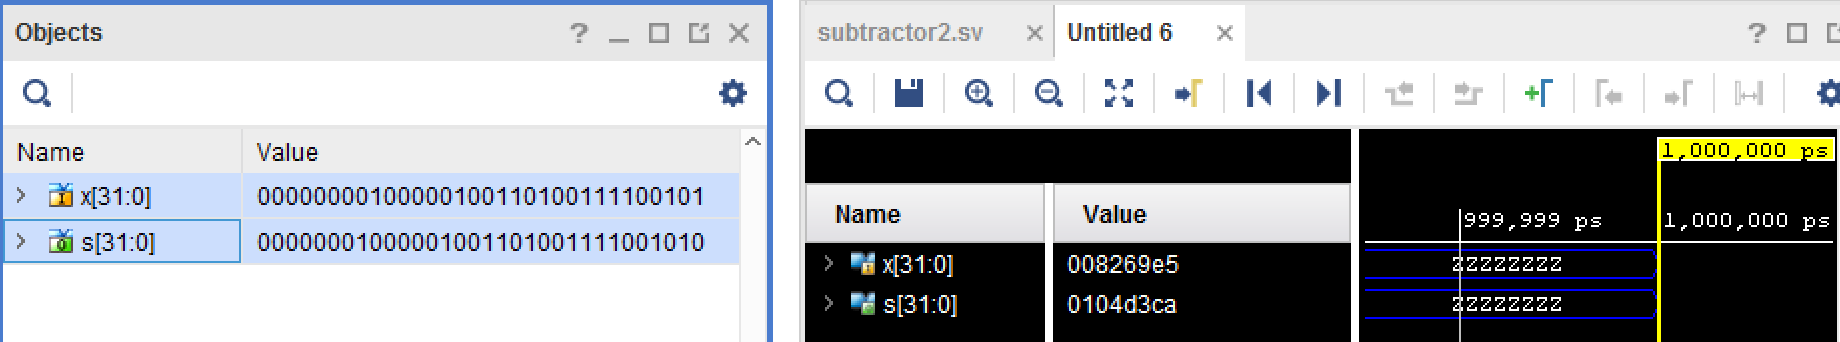
\includegraphics[scale=0.5]{photos/shleft_simulation}
\break
The 1-bit logical shift process takes in A as a 32-bit input and performs a 1-bit shift left on A. The result of the shift is then stored into the return output S, which in turn would be the final return value for Out in the main module calling this ShiftLeft module.

\subsection{SIMD Add: Four 8-bits Add}
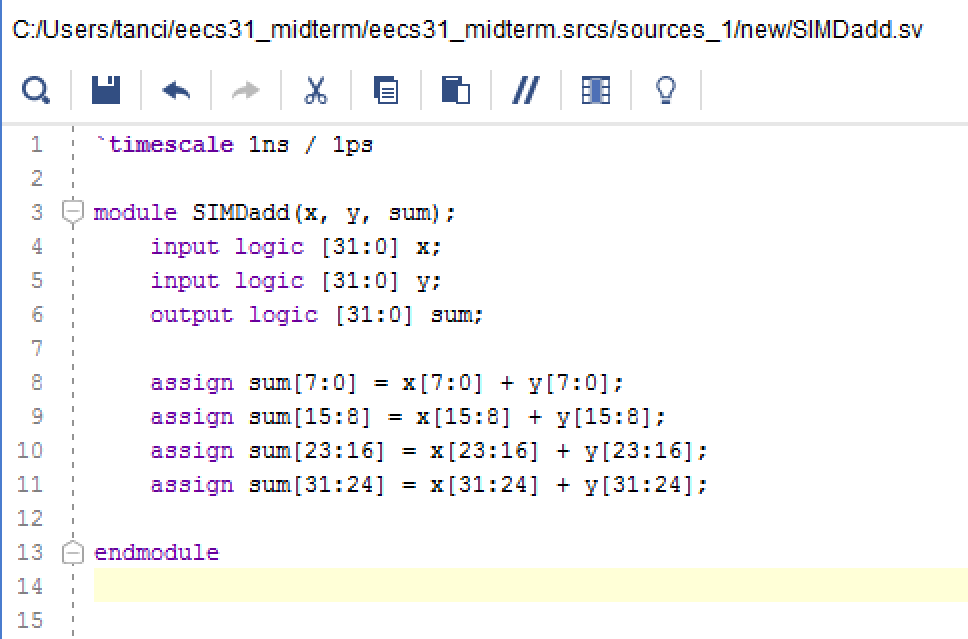
\includegraphics[scale=0.5]{photos/SIMDadd_code}
\break
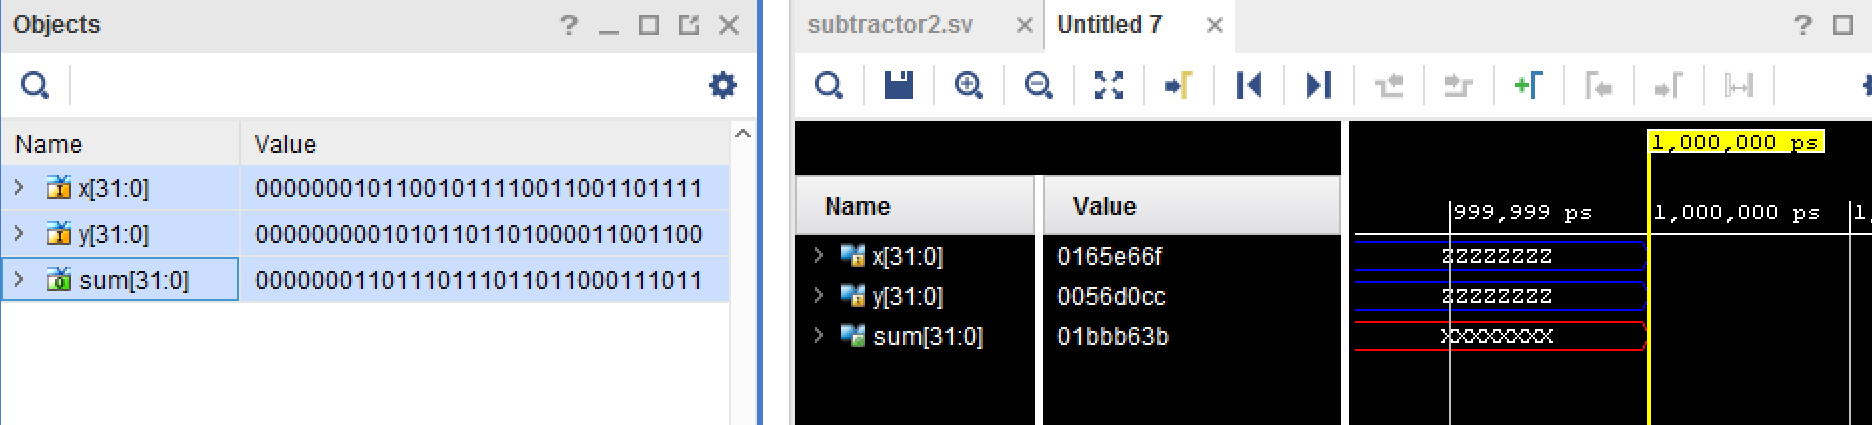
\includegraphics[scale=0.5]{photos/simdadd_simulation}
\break
The SIMD Add module takes in two input 32-bit values x and y, and one 32-bit output return sum. Every 8-bits of x and y are added and stored into the corresponding 8-bit location in sum, carry outs ignored as it will not be stored into the resultant sum. Concatenation was an initial idea to saving the result of every 8-bit addition into the resultant output variable, but saving the values directly into an allocated 8-bit area would already directly alter the values in the output variable, therefore a direct assignment was used instead of concatenation for ease in the code. Carry out is ignored because it is out of bounds for the storage space. This module was tested using values where carry out was ensured but not carried over at every 4 bits:
x and y as {8{4'b1000}}, resulting in 0001000000010000000100000010000, and x = 10110111 00111010 11100010 01101100, y = 10010010 10010010 00101001 10100010 resulting in 01001001110011000000101100001110.

\subsection{Bitwise AND}
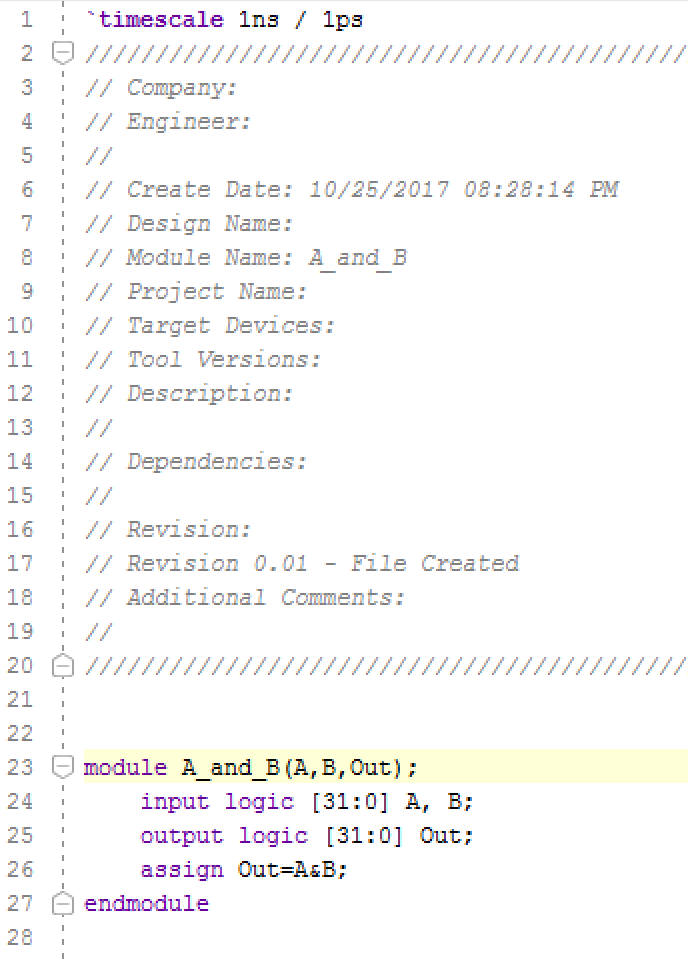
\includegraphics[scale=0.5]{photos/and_code}
\break
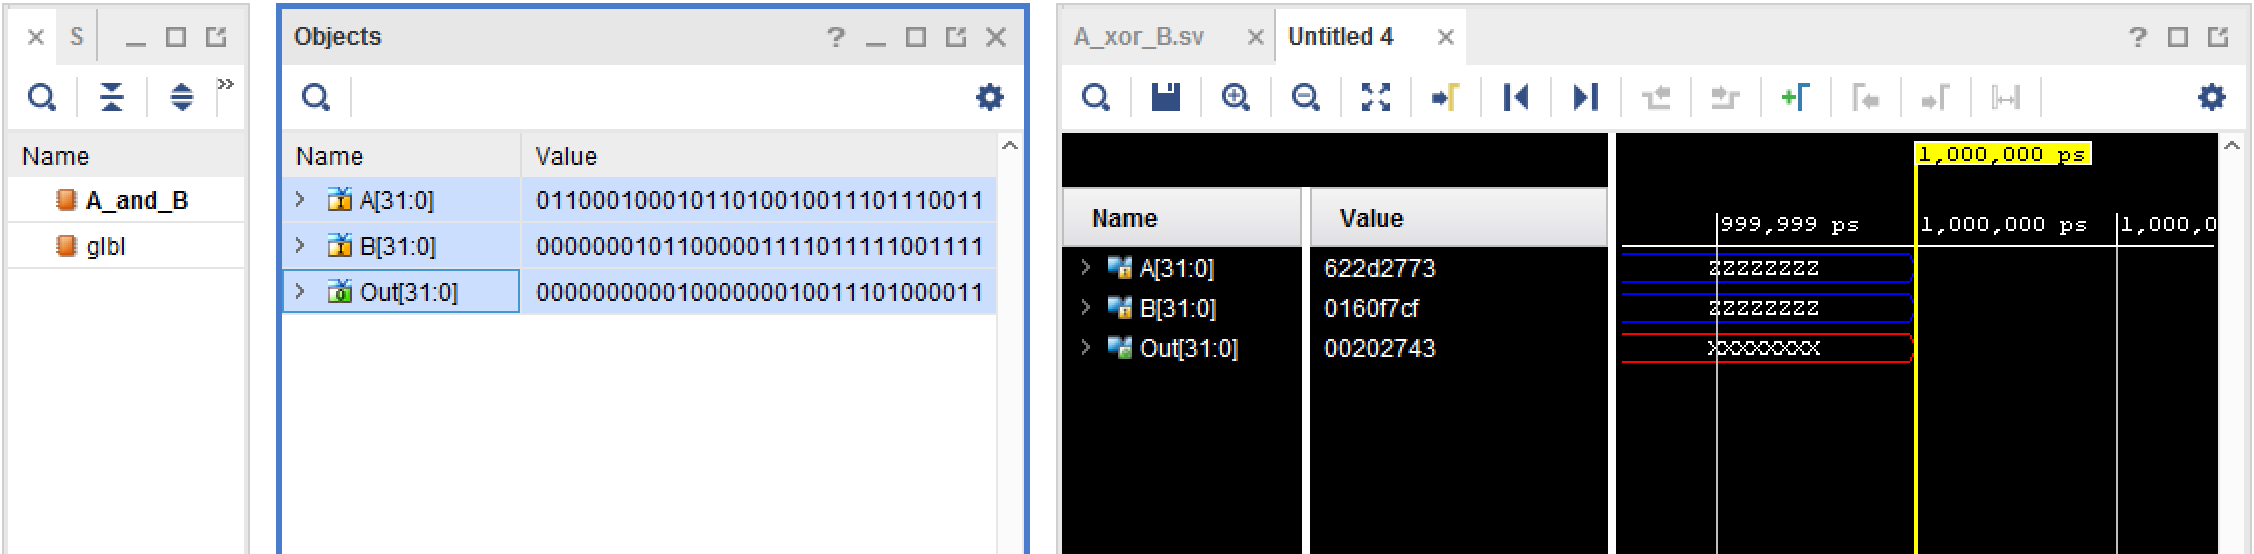
\includegraphics[scale=0.4]{photos/and_simulation}
\break
The bitwise AND module compares two inputted 32 bit numbers and returns either 1 or 0 for each compared bit depending on the given values by using the "\&" operator. If there is a 0 the module it returns 0 but otherwise returns 1, following the digital logic AND operation described in class. The code was tested with multiple values including {32'b0} and {1011, 28'b1} before concluding it was accurate.

\subsection{Bitwise OR}
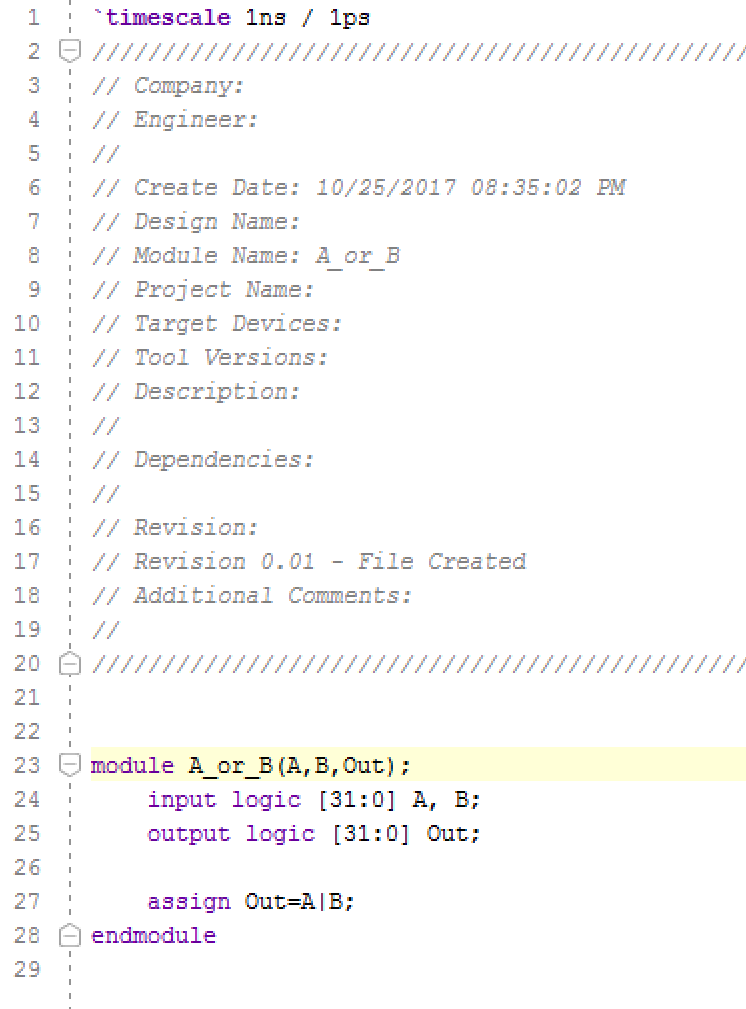
\includegraphics[scale=0.5]{photos/or_code}
\break
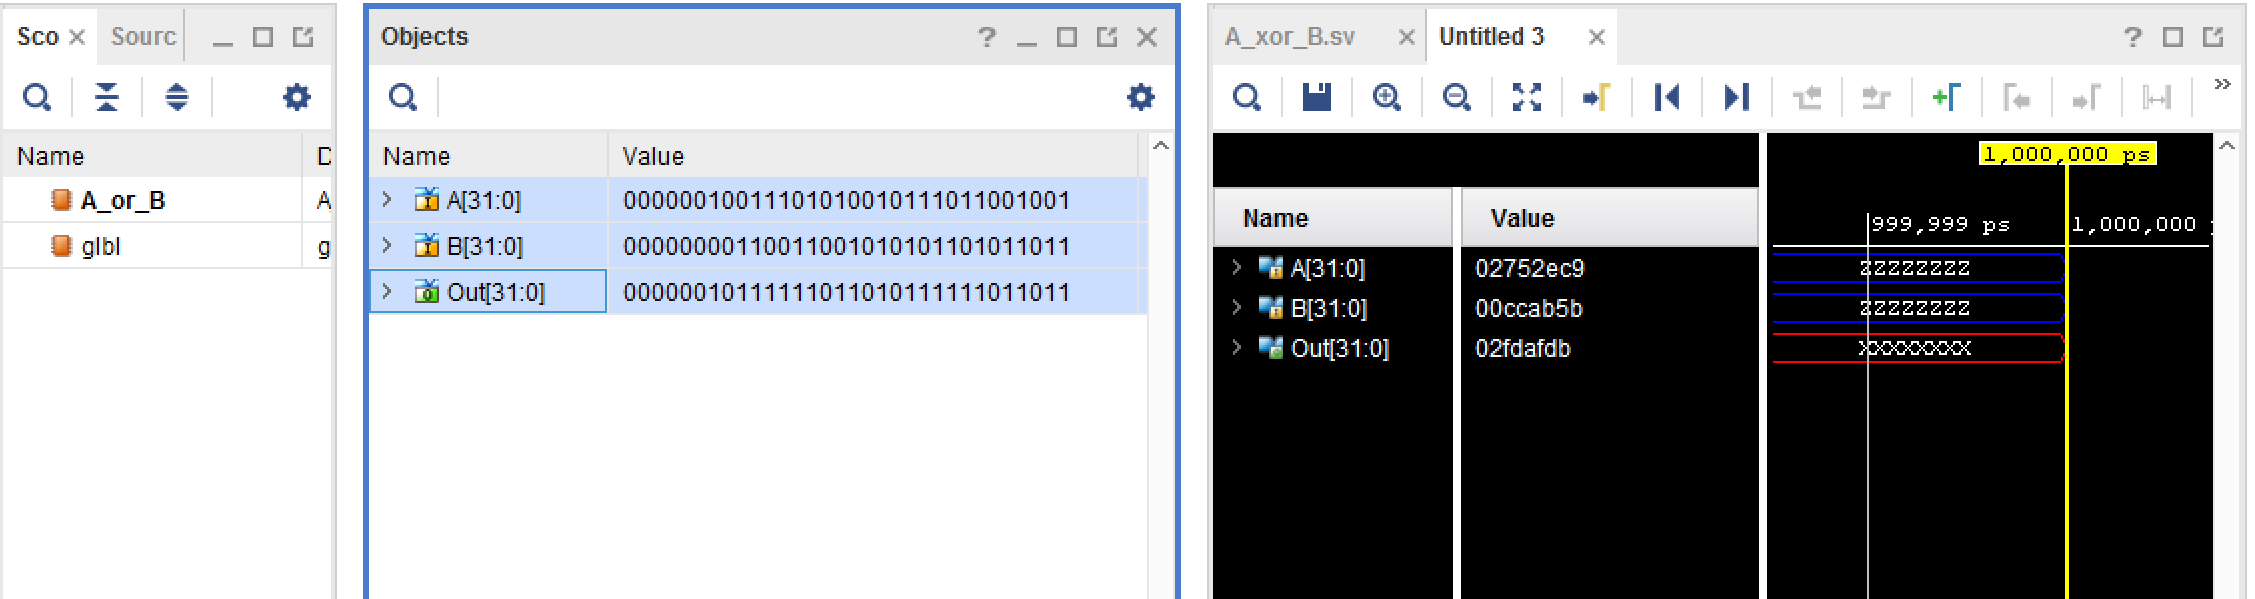
\includegraphics[scale=0.4]{photos/or_simulation}
\break
The bitwise OR module compares two inputted 32 bit numbers and returns either 1 or 0 for each compared bit depending on the given values. By using "|", the operator returned 1 if the two bits being compared had a 1 present, otherwise it returned 0. This followed the OR digital logic definition explained in class and after testing the code with both basic values like {32'b0} and {32'b1} as well as {111,29b'0} and {1001, 28b'1} the code was considered successful.

\subsection{Bitwise XOR}
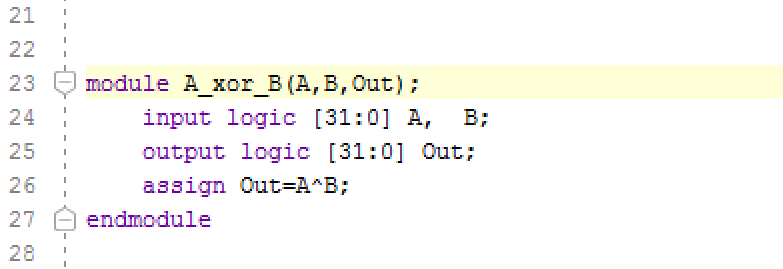
\includegraphics[scale=0.5]{photos/xor_code}
\break
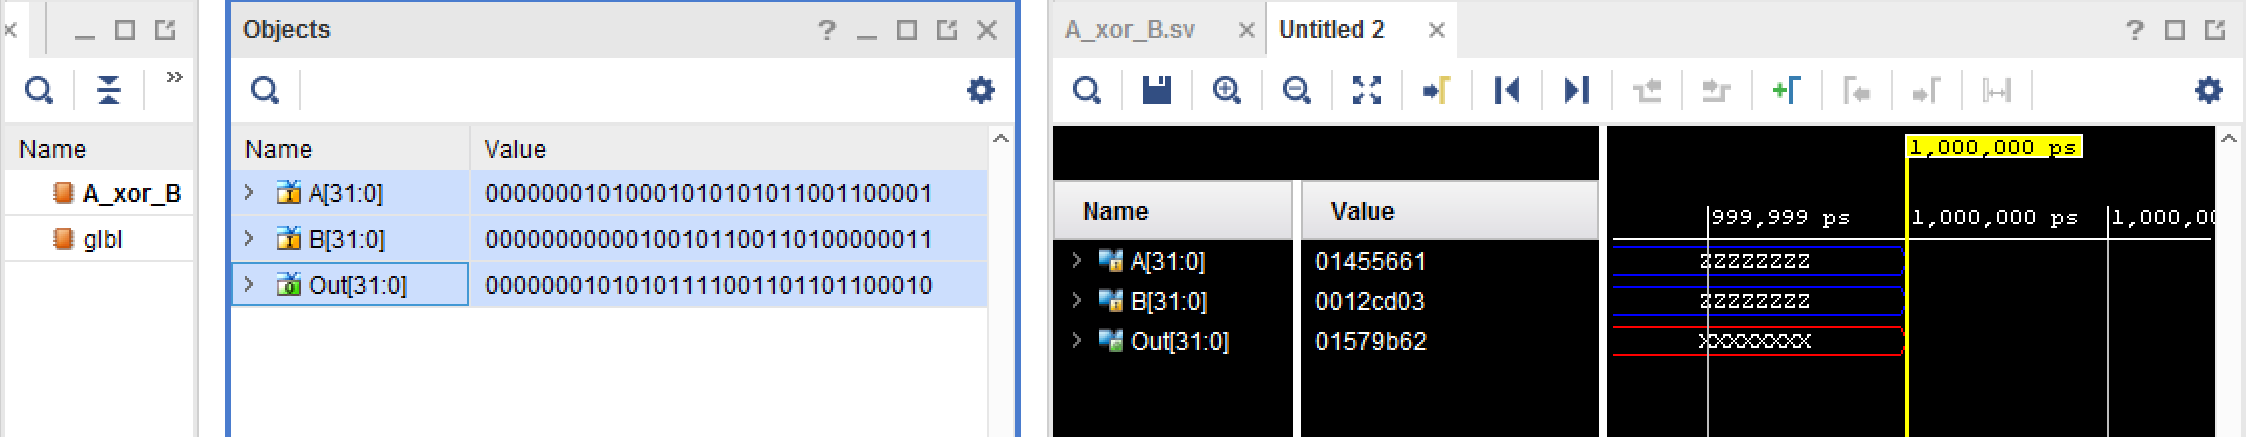
\includegraphics[scale=0.4]{photos/xor_simulation}
\break
According to the definition of XOR, if the two bits being compared are the same (either both 1 or both 0) then it returns 0. Otherwise, if only one of the bits is 1, XOR returns 1. By using the XOR operator, \^ \, the module traverses the index of the first given value with the corresponding index of the second value. After testing values, like {25b'1, 0101110} and {29b'0, 3b'1}, the code seemingly accomplished it's goal.

\subsection{Complement}
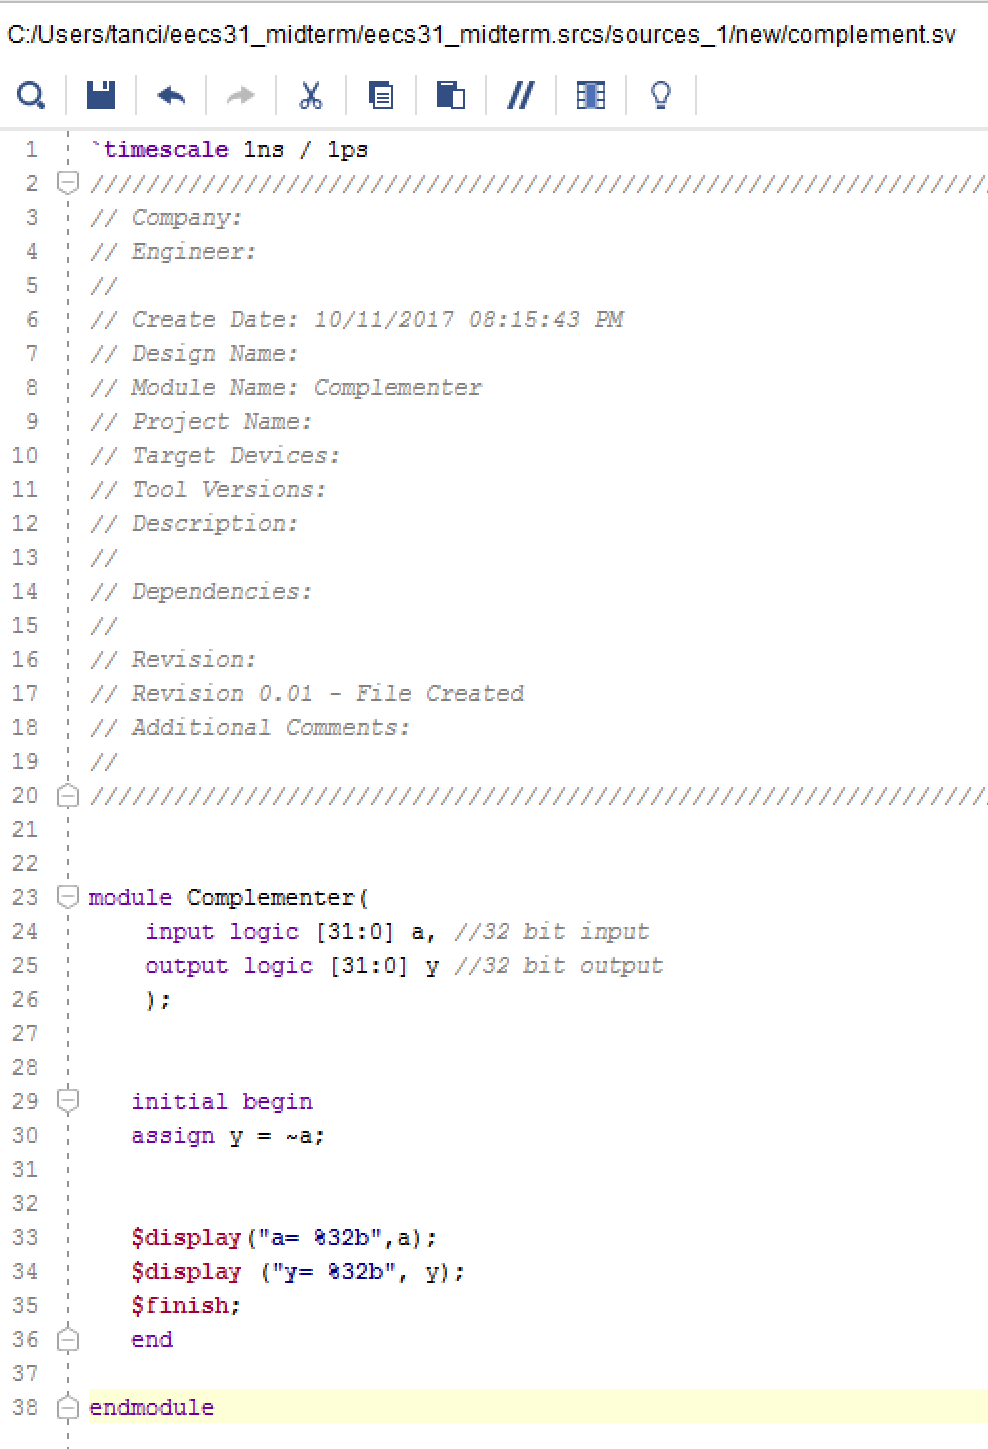
\includegraphics[scale=0.5]{photos/complementer_code}
\break
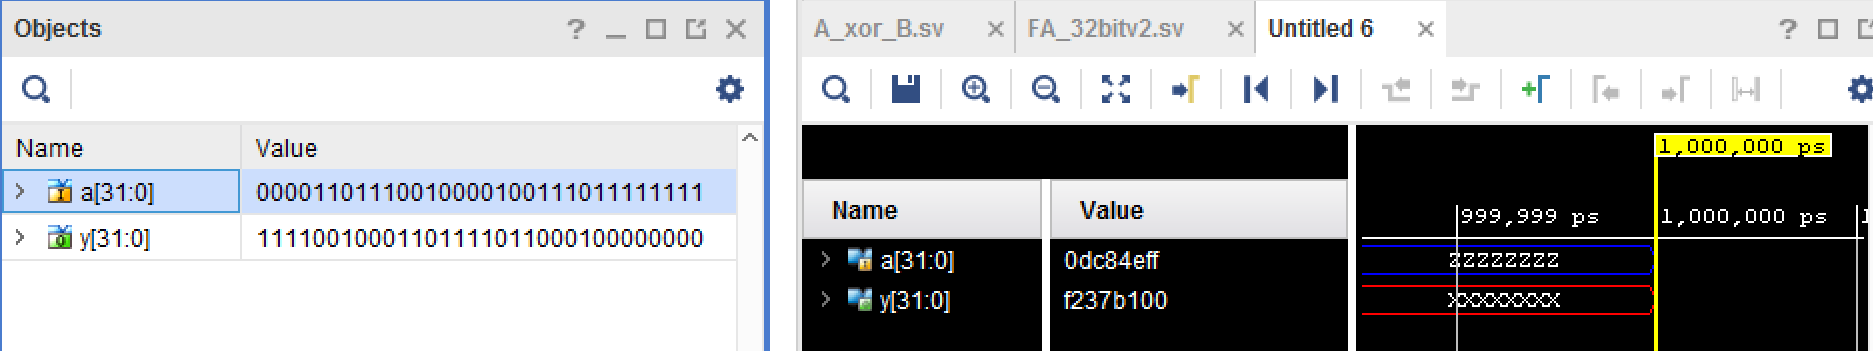
\includegraphics[scale=0.5]{photos/complimenter_simulation}
\break
The Complement process takes the user 32 bit input and inverts the inputs. For instance, if the user inputs a binary number for a[31:0] with \\ 00000000000000010000000000000001, we would expect the output of y[31:0] the complement to be 11111111111111101111111111111110. This is implemented in SystemVerilog by inverting the 1's to 0's and vice versa as show in the image below. To implement this in SystemVerilog, we define one input port and one output port. We assign the output y as the NOT of the input a. 


\subsection{2's Complement}
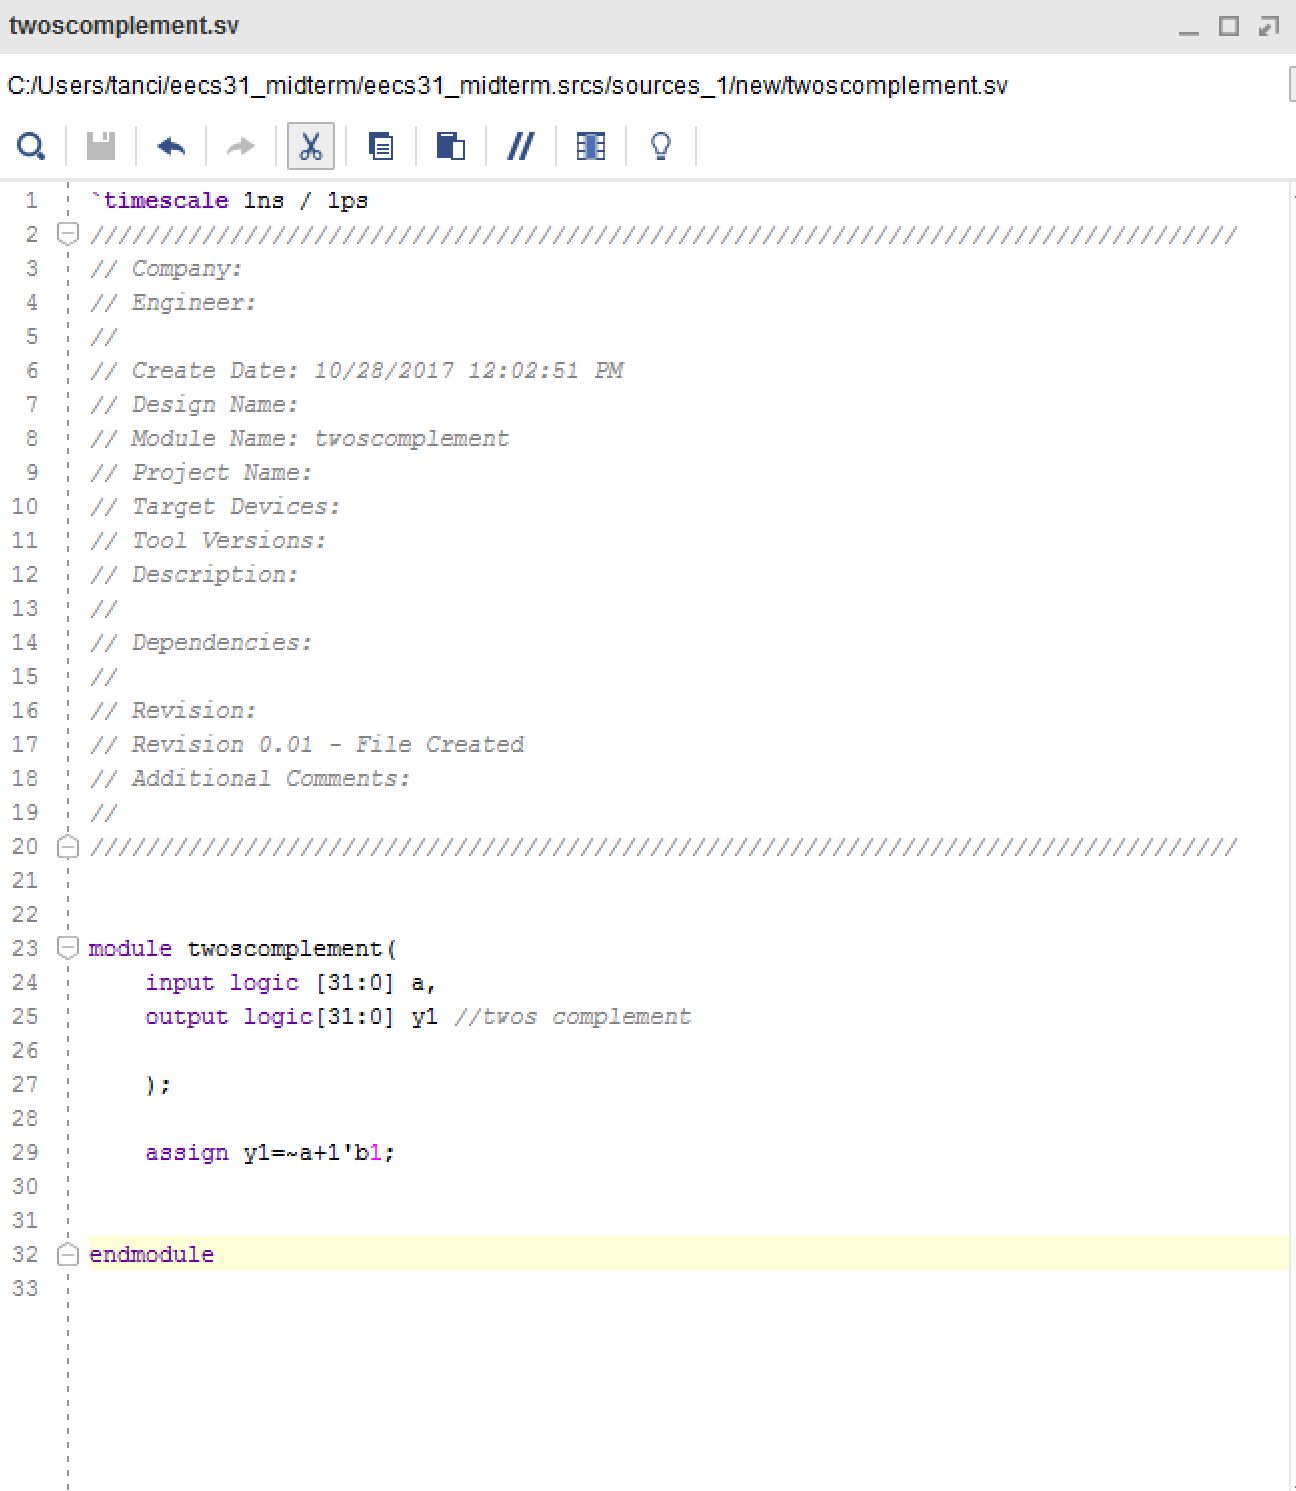
\includegraphics[scale=.50]{photos/twoscomplement_code}
\break
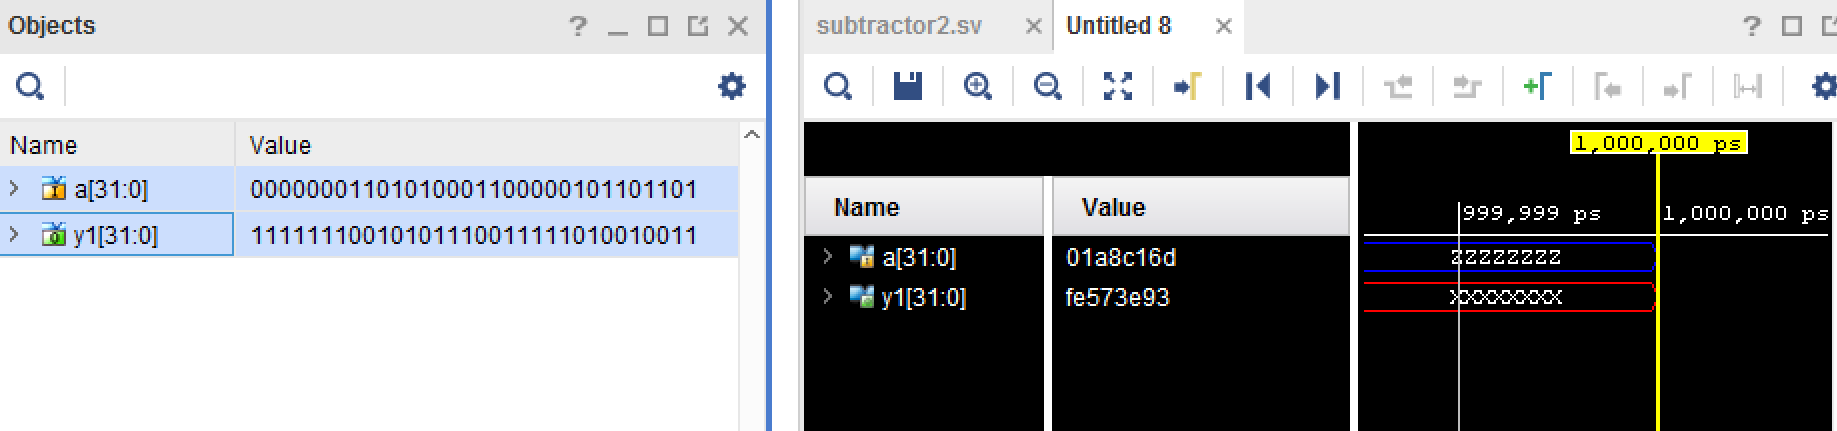
\includegraphics[scale=.5]{photos/twocomplement_simulation}
\break
The 2's Complement process takes the 32 bit input to get the complement and then add 1 to get 2's complement. For instance, if the user inputs \\ 00000000000000000000000000001111 then the complement would be \\ 11111111111111111111111111110000. With the complement, we would add 1 to the complement to get 11111111111111111111111111110001 which is what we would expect the output would be when implementing the code on SystemVerilog. To implement this in SystemVerilog, we define one input port and one output port. We assign the output as the NOT of the input plus 1 to simulate the two's complement.

\subsection{Main Function and Multiplxer}
In order to fully impliment the code to simiulate as one unit, the UM group created a main source code that will instantiate all of the previously explained functions, along with a multiplexer(MUX). The inputs of this function are two 32 bit numbers. The outputs are a 32 bit final output, 1 bit carry flag, 1 bit sign flag, 1 bit overflow flag, and a 1 bit zero flag. In addition, there are also 12 temporary value holders that correspond the outputs of each function of the Enhanced ALU and 2 temporoary values for the carry and sign flag. When run, the main fucntion will instatiate all functions at once, the final outputs and flags will be determined through the use of the multiplexer.\newline\newline The multiplexer functions as a case assignment statement, using 12 temporary varibales that correspond to each function of the Enhanced ALU, the MUX uses the value of the selector bits to assign the appropriate value to the final output. There is another case assignment statement that is used to assign the correct values for the overflow and sign flag. Previously there was a problem found in the project that would produce an "x" value. This was found to be from the assignment of the same variable to two differnet instatiantions. This flag case assignment will only produce a value for the selected addition or subtraction function, otherwise it will be "x".
\section{Implementation and Bit-stream transfer to \\ FPGA}
Since the FPGA board does not possess the ability to appropriately display 32 bits, it becomes necessary to alter the inputs in a way that the board will work appropriatley with the Enhanced ALU. This was done by redefining the inputs and output as a 6 bit number instead of a 32 bit number. In the main function code, there are 2 new values that would be defined as 32 bit numbers and take in the values of the inputs which are concatenated with twenty-six 0's. These new values place hold the values of the 6 bit inputs so that the rest of the modules would not have to be altered. A new variable was also assigned and would be the output variable in all the instatiations. The 31 bit to the 26 bit of this number would then be assigned to the 6 bit main output. \newline\newline Once the board was synthesized and the bit stream was generated, it was observed that the FPGA was able to diplay most of the functions. Some functions that could not be appropriatley dispalayed on the FPGA are the increment and decrement functions. This was found to not be an error in the code, but a lack of defined ability. The increment and decrement cannot be ovbserved on the FPGA using this code, however simulations state that it is functional.

\section{Conclusion}
Ultimately, the Enhanced ALU was designed and simulated with concepts and formulated equations learned previously through block diagrams and Karnaugh Maps. For much of this project, trial and error helped guide the approach for each ALU operation towards efficiency and modularity. Building on the concepts known already about multiplexers, ALUs, bit-manipulation, and other arithmetic functions, we learned to implement this to the Enhanced ALU and practiced in SystemVerilog.

\end{document}